\documentclass[12pt,oneside,noprintercorrection]{iut}
\usepackage[utf8]{inputenc}
%----------------------------------------------------------------------
%                     Chargement de quelques packages
%----------------------------------------------------------------------

% Si l'on produit le PDF avec pdflatex, ceci remplace la plupart
% des polices EC par des polices CM, plus adaptees a la generation de PDF,
% car ayant des equivalents PS :

\usepackage[cyr]{aeguill}

% pour les includegraphics
\usepackage{graphicx}

% mini "table of content"
\usepackage[french]{minitoc}
\usepackage[french]{babel}


% couleur des liens et hyperref -> mettre à {0.0,0.0,0.0} pour avoir du noir
%                               -> mettre à {0.2,0.2,0.2} pour avoir du gris foncé
\usepackage{color}
\definecolor{linkcolor}{rgb}{0.1,0.1,0.7}
\usepackage[hypertexnames=false]{hyperref}
\hypersetup{
    colorlinks,%
    citecolor=linkcolor,%
    filecolor=linkcolor,%
    linkcolor=linkcolor,%
    urlcolor=linkcolor,%
}

% Pour les codes
\usepackage{listings}
\lstset{language=C++,basicstyle=\small}


\usepackage{silence}

\WarningFilter{minitoc(hints)}{W0023}
\WarningFilter{minitoc(hints)}{W0024}
\WarningFilter{minitoc(hints)}{W0028}
\WarningFilter{minitoc(hints)}{W0030}
\WarningFilter{hyperref}{bookmark level}

\WarningFilter{blindtext}{} % this takes care of the `blindtext` messages

%-------------------------------------------------------------------
%  Surcharge de commandes pour les variables et page d'en-tête
%-------------------------------------------------------------------

\makeatletter

%
% les deux commandes suivantes sont entre \makeatletter
% et \makeatother parce qu'elles utilisent des `@'.
%

\renewcommand{\@DFD}{Universit\'e Polytechnique des Hauts de France\\}


\renewcommand{\@Lillehe@d}{{\UseEntryFont{ThesisFirstPageHead}\noindent
    \centerline{\if@logo@uhp@
                    {\setbox0=\hbox{$\raise2.3cm\hbox{\UHPLogo}$}%
                     \ht0=\baselineskip\box0}\hfill
                \else
                    Universit\'e Lille%
                \fi}%
    \@TL@cmn@head\\
    \par
    }%
    }


\newcommand\TheseLilleI{\renewcommand{\@ThesisFirstPageHead}{\@Lillehe@d}%
                         \ThesisDiploma{{\UseEntryFont{ThesisDiploma}%
                              \\[3mm]
            {\UseEntryFont{ThesisSpecialty}( )}}}}

\makeatother

%-------------------------------------------------------------------
%           Corrections pour les imprimantes recto-verso
%                          (A AJUSTER)
%-------------------------------------------------------------------

%\ShiftOddPagesRight{-1mm}
%\ShiftOddPagesDown{2.5mm}
%\ShiftEvenPagesRight{0mm}
%\ShiftEvenPagesDown{0mm}

%-------------------------------------------------------------------
%                Mise en page
%-------------------------------------------------------------------

%-------------------------------------------------------------------
%                             interligne
%-------------------------------------------------------------------
\renewcommand{\baselinestretch}{1.3}

%-------------------------------------------------------------------
%                             Marges
%-------------------------------------------------------------------

% pour positionner les vraies marges:
%\SetRealMargins{1mm}{1mm}

%-------------------------------------------------------------------
%                             En-tetes
%-------------------------------------------------------------------
%On n'utilise pas les logos
%\DontShowLogos

% Les en-tetes: quelques exemples
%\UppercaseHeadings
%\UnderlineHeadings
%\newcommand\bfheadings[1]{{\bf #1}}
%\FormatHeadingsWith{\bfheadings}
%\FormatHeadingsWith{\uppercase}
%\FormatHeadingsWith{\underline}
\newcommand\upun[1]{\uppercase{\underline{\underline{#1}}}}
\FormatHeadingsWith\upun

\newcommand\itheadings[1]{\textit{#1}}
\FormatHeadingsWith{\itheadings}

% pour avoir un trait sous l'en-tete:
\setlength{\HeadRuleWidth}{0.4pt}


%-------------------------------------------------------------------
%                         Les references
%-------------------------------------------------------------------

\NoChapterNumberInRef \NoChapterPrefix

%-------------------------------------------------------------------
%                           Brouillons
%-------------------------------------------------------------------

% ceci ajoute une marque `brouillon' et la date
%\ThesisDraft




\renewcommand{\labelitemi}{$\bullet$}
\renewcommand{\labelitemii}{$\circ$}
%-------------------------------------------------------------------
%                          Encadrements
%-------------------------------------------------------------------

% encadre les chapitres dans la table des matieres:
% (ces commandes doivent figurer apres \begin{document}

%\FrameChaptersInToc
%\FramePartsInToc


%-------------------------------------------------------------------
%            Reinitialisation de la numerotation des chapitres
%-------------------------------------------------------------------

% Si la commande suivante est presente,
% elle doit figurer APRES \begin{document}
% et avant la premiere commande \part
\ResetChaptersAtParts

%-------------------------------------------------------------------
%               mini-tables des matieres par chapitre
%-------------------------------------------------------------------

% preparer les mini-tables des matieres par chapitre.
% (commande de minitoc.sty)
%\dominitoc

\NewJuryCategory{EncadrantEts}{\it Encadrant entreprise :}{\it Encadrant entreprise:} 
\NewJuryCategory{EncadrantUniv}{\it Encadrant universitaire :}{\it Encadrant universitaire:} 

\TheseLilleI


% Commandes macros de raccourcis
\newcommand{\glaz}{Glaz tech+fi}
\newcommand{\gz}{Glaz}
\newcommand{\slf}{Salesforce}
\newcommand{\fa}{Form Assembly}




%-------------------------------------------------------------------
%                         Page de titre:
%-------------------------------------------------------------------


\ThesisTitle{Aider les analystes financiers à numériser leur travail avec Salesforce}
\ThesisKind{Rapport de stage}
\ThesisPresentedThe{soutenu le 27/06/2023}
\ThesisAuthor{Sacha DON}

\NomDuLaboOuEntreprise{\glaz{}}
\LogoLaboOuEntreprise{img/logoglaz.png} % Image du logo du labo ou ets dans le rep img

\EncadrantEts = {Antoine Laudet}
\EncadrantUniv = {Mustapha Ratli}

\begin{document}

% Creation de la page de titre:
\MakeThesisTitlePage



%-------------------------------------------------------------------


%-------------------------------------------------------------------
%                          remerciements
%-------------------------------------------------------------------

%\DontFrameThisInToc
\begin{ThesisAcknowledgments}
Je voudrais avant tout remercier toute l'équipe de \glaz{}. Notamment Monsieur Samuel MINNE, mon tuteur, Quentin PROGNON, alternant en Master E-Services et chef du projet sur lequel j'ai travaillé,  Zo Tahina RATEFIARIVONY, alternant en Master Génie Logiciel, Louise DELBECQUE, alternante en Master E-Services, Abdelkader AMARA, alternant en Master E-Services également, Anis SAHED, alternant en MIAGE, Kenneth MAGNAGNA, alternant en études de finance de marché trading, Néo LEFRANC, stagiaire en Licence Informatique et Antoine LAUDET, le dirigeant de l'entreprise, qui m'ont fait confiance, m'ont gracieusement accueilli mais qui m'ont surtout encadré et aidé tout au long de cette année d'alternance.
J'aimerais également remercier Monsieur Mustapha RATLI qui m'a suivi durant cette année d'alternance.
\end{ThesisAcknowledgments}





%-------------------------------------------------------------------
%                  ecriture de `Chapitre' et `Partie'
%                      dans la table des matieres
%-------------------------------------------------------------------

\WritePartLabelInToc \WriteChapterLabelInToc


%-------------------------------------------------------------------
%                        table des matières
%-------------------------------------------------------------------

\tableofcontents

%-------------------------------------------------------------------
%              Exemple d'utilisation de \SpecialSection
%-------------------------------------------------------------------

% La commande \mainmatter (nouvelle commande LaTeX2e) permet de passer
% a la numérotation arabe (ce que fait \pagenumbering{arabic})
% et de faire commencer la nouvelle page 1 sur une page impaire.
% On evitera donc d'utiliser directement \pagenumbering{arabic}.
\mainmatter

% ----------------------------------------------------------------
\SpecialSection{Introduction}
Dans le cadre de ma formation en Licence professionnelle Développement Web et Mobile, j'ai eu l'opportunité d'effectuer une alternance au sein de l'entreprise \glaz{}. Cette expérience m'a permis de mettre en pratique les connaissances acquises lors de ma formation, mais aussi de développer de nouvelles compétences en travaillant sur des projets concrets et stimulants.

L'entreprise Glaz Tech +Fi est spécialisée dans le développement de solutions technologiques innovantes. Parmi ses réalisations, le Shaker Data se distingue comme un outil essentiel de l'entreprise. C'est un véritable allié pour les professionnels du secteur financier, tels que les analystes financiers, les gestionnaires de patrimoine ou encore les courtiers immobiliers. Le Shaker Data est conçu pour recueillir et analyser les informations des clients, permettant ainsi d'évaluer la faisabilité de crédits bancaires. L'objectif est de proposer des produits bancaires sur mesure, parfaitement adaptés aux besoins spécifiques de chaque client.

Durant mon alternance, j'ai eu le privilège de contribuer au développement et à la maintenance du Shaker Data. Cette expérience m'a permis non seulement de comprendre le fonctionnement interne de cet outil, mais aussi de participer activement à son amélioration et à son évolution.

Ce rapport présente en détail les activités que j'ai menées au cours de mon alternance, les compétences que j'ai acquises et les leçons que j'ai tirées de cette expérience enrichissante.

Dans la première partie de ce rapport, je présenterai Glaz Tech +Fi et expliquerai en détail le rôle du Shaker Data au sein de l'entreprise. Ensuite, je décrirai la méthode et les moyens que j'ai utilisés pour développer et maintenir l'outil. La troisième partie sera consacrée à la présentation des résultats de mon travail et des apports de celui-ci. Enfin, je conclurai en soulignant les contributions significatives de mon travail à l'entreprise, en mettant en évidence les compétences et les connaissances que j'ai acquises au cours de cette expérience.

% Pour ne paœur du s avoir le mot `Chapitre' au debut de chaque chapitre.
\NoChapterHead

\chapter{Comprendre \glaz{} et le Rôle du Shaker Data}
\section{\glaz{}}

\glaz{}, forte de plus de 20 ans d'expertise en solutions financières, a su s'adapter aux évolutions technologiques et informatiques pour se réinventer en tant que Fintech. Collaborant avec des acteurs financiers tels que des gestionnaires de patrimoine, des analystes financiers et des courtiers immobiliers, l'entreprise a réussi à numériser ses processus métiers grâce à l'intégration de Salesforce. Cette transformation a marqué un tournant significatif pour Glaz Tech +Fi, qui a su allier avec brio l'analyse financière et l'informatique.

\gz{} se consacre à fournir à ses clients des solutions financières adaptées à leurs besoins spécifiques de financement. Pour atteindre cet objectif, l'entreprise a établi plusieurs mandats avec diverses banques. Ces mandats permettent non seulement à Glaz Tech +Fi de proposer des solutions financières personnalisées à ses clients, mais aussi de comprendre en profondeur les spécificités de chaque produit financier.

En tant que mandataire de banque, le rôle de \glaz{} est d'accompagner ses clients tout au long de leur parcours de financement. Cela comprend la préparation du dossier de financement jusqu'à la signature finale du contrat.

Actuellement, \gz{}, en tant que mandataire de banque, propose des solutions de financement pour trois types de projets principaux : les projets de financement immobilier, le rachat de crédit, et l'acquisition de parts de Sociétés Civiles de Placement Immobilier (SCPI).

L'entreprise se compose de deux équipes complémentaires : une équipe financière et commerciale basée à Ploemeur, en Bretagne, et une équipe informatique située à Lille. Cette configuration permet une communication constante et efficace entre les deux équipes, essentielle pour définir conjointement les besoins, suivre les évolutions et corriger les éventuels bugs.

Glaz Tech +Fi se distingue par son processus d'analyse de dossiers de financement provenant d'apporteurs d'affaires, notamment des conseillers en gestion de patrimoine, des courtiers immobiliers, ou bien des analystes financiers. Une fois le dossier reçu, l'entreprise réalise une analyse approfondie de sa faisabilité. La qualité de cette analyse est largement reconnue, tant par les apporteurs d'affaires que par les banques partenaires, attestant de l'expertise et de la fiabilité de Glaz Tech +Fi.

\clearpage

\subsection{L'équipe financière et commerciale}
Je vais d'abord vous présenter l'équipe financière de l'entreprise. Je peux premièrement vous parler d'Antoine Laudet qui est le dirigeant de l'entreprise. C'est lui qui nous partage sa vision sur le modèle économique et nous transmet et reformule les besoins des clients avec qui il est en contact. C'est à lui que l'on montre les avancées de nos projets et c'est également lui qui nous guide par rapport aux évolutions à y apporter. Ensuite, nous avons Aurélie Kerlir, la responsable de l'équipe d'analyse, qui est là pour nous apporter une idée des correctifs ou des améliorations à réaliser sur les différents projets de l'entreprise. Avec Stephen Gouzouguen, le directeur commercial, ils vont nous faire parvenir les retours des utilisateurs, mais également les problèmes qu'ils ont rencontré voire encore même des idées d'améliorations.
Pour ce qui est de l'aspect des Ressources Humaines, Isabelle est la personne à qui il faut s'adresser si on a un problème humain.


\subsection{L'équipe informatique}
Pour ce qui est de l'équipe informatique dont j'ai fait partie, Samuel Minne est le chef technique de l'équipe, c'est donc vers lui que l'on va se tourner en général lorsqu'il y a un problème. Il développe, mais prend également en charge la direction technique des différents projets de l'entreprise. Ensuite, nous avons Oliver Irwin et Tristan Coignion qui sont deux alternants, tous les deux en deuxième année de Master, le premier en Machine Learning, le second en Génie Logiciel. Les deux étant alternants chez \gz{} depuis 2 ans, ils ont beaucoup plus d'expérience que moi sur l'environnement de travail utilisé par \gz{}, mais également sur la programmation en elle-même. Oliver est le chef de projet de "Gespat" et je suis donc en collaboration directe avec lui sur le projet. Tristan, quant à lui, est en charge du projet "Shaker Data Light". Ainsi, avec leur expérience et leur savoir-faire, ils ont pu avec Samuel, me guider et m'aider sur la prise en main des outils utilisés par l'entreprise, mais également lors de moments où j'étais en difficulté et avais besoin d'aide sur mon code. Ils ont tous les deux un rôle de développeur, mais ont plus de responsabilités que les autres développeurs de par leur expérience et leur niveau d'études. L'équipe est également composée de Quentin Prognon et de Louise Delbecque, qui sont en première année de Master E-Services et également alternants chez \gz{}. Quentin, ayant fait son stage de troisième année de licence informatique chez \gz{}, a assez d'expérience pour pouvoir m'aiguiller sur certains points et a pu me venir occasionnellement. Louise, a pu également quelquefois m'aider et m'éclairer. Enfin, Zo Tahina Ratefiarivony et Abdelkader Amara, sont arrivés dans l'entreprise quasiment en même temps que moi.  Ce sont deux étudiants qui sont en 3e année de licence informatique. Ainsi, nous formons un trio de stagiaire, et nous prenons chacun un rôle de développeur \slf{}.

\subsection{Les projets de \glaz{}}
\subsubsection{Shaker Data}
Cet outil est le principal de \gz{}. Il permet de calculer la faisabilité d'un projet d'un client en fonction du besoin de financement du projet, et des revenus et de la situation financière du client. Ainsi, à la fin de la saisie des données d'un client par les gestionnaires de patrimoine ou les courtiers utilisant l'outil, le Shaker Data va indiquer si ce client est éligible à ses demandes, sinon, l'outil lui explique les différentes raisons du refus de son éligibilité. Toutefois, Shaker Data va l’orienter sur les démarches à suivre afin de requalifier son dossier dans le but de le rendre éligible. Avec cet outil, cela évite aux analystes financiers de devoir faire plusieurs calculs redondants et lourds, avec Shaker Data, les analystes n'ont plus qu'à remplir les données de leurs clients.

\subsubsection{Shaker Reader}
Cet outil utilise un agrégateur de compte bancaire. Cela permet donc de regrouper sous une seule interface plusieurs comptes détenus par un seul et même client. Shaker Reader permet également de faire gagner du temps sur l'analyse de dossier d'un client. En effet, les données financières du client étant déjà en partie analysées, cela permet de récupérer et de calculer des métriques intéressantes automatiquement via l'outil, qui seraient très encombrantes et redondantes à calculer à la main. Ces calculs permettent notamment pour l'analyste de voir le nombre de jours à découvert, le solde journalier ou encore les différentes catégories de dépense et de revenus du client.  Ainsi, les analystes ont une vision globale des finances de leurs clients, et peuvent analyser plus facilement les comptes du client, au lieu de devoir éplucher un par un chaque compte et chaque relevé bancaire.
\clearpage

\section{Le Shaker Data}
L'entreprise a pu voir le besoin d'un outil facilitant le travail des gestionnaires de patrimoine lors de sa présence au salon ``Patrimonia'', qui est le plus grand rassemblement en France des professionnels de l’univers du conseil patrimonial. La vision de ce besoin a provoqué une étincelle chez \gz{}, et l'entreprise a donc voulu saisir l'opportunité en ayant pour projet de concevoir et développer cet outil. Étant donné que \gz{} avait déjà beaucoup de projets en construction, il était nécessaire de recruter. L'entreprise a donc recruté 3 stagiaires dont moi-même, dans le but de les former à \slf{}, afin d'ensuite lancer notamment le projet "Gespat". Cela permet d'entrevoir une possibilité d'évolution pour les stagiaires. En effet, l'entreprise a recruté 3 stagiaires voulant éventuellement évoluer vers une alternance au sein de l'entreprise. Cela permettrait d'obtenir une continuité du suivi des projets pour \gz{}, mais également pour les stagiaires. Les raisons qui m'ont poussé à accepter de faire ce stage chez \glaz{}, est le fait qu'il était nécessaire de réaliser un stage pour valider ce 4e semestre de DUT, mais également au fait que j'aime le monde de la finance. Si je n'avais pas étudié dans le domaine de l'informatique, j'aurais  en effet choisi celui de la finance.

\section{Les technologies utilisées par \gz{}}
\subsection{Salesforce}
La technologie principale utilisé par \glaz{} est \slf{}. \slf{} étant un outil de gestion de relation client, qui plus est le numéro un mondial sur le marché, il est l'outil idéal pour \gz{}. En effet, c'est la problématique principale de l'entreprise, elle cherche à simplifier la gestion et les démarches, pour les partenaires externes et pour les analystes internes présents dans l'entreprise. \slf{} a donc logiquement permis à \gz{} d'effectuer sa transformation numérique.
~\\\indent \slf{} est une sorte de Framework permettant d'éditer des logiciels. \slf{} contient donc une base de données embarquée, en corrélation avec la gestion de relation client, mais qui est personnalisable.
Un outil de modification de page grâce à un glisser-déposer est également présent dans \slf{}. Il permet de personnaliser les différentes pages de notre application. En résumé, \slf{} est une sorte de plateforme d'hébergement d'applications, avec tous ses outils de développement et sa base de données qui vont avec.

\subsubsection{Apex}
La plateforme de développement de \slf{} utilise le langage orienté objet qu'est Apex. C'est un langage qui se rapproche grandement du Java et qui en est inspiré. Pour pouvoir déployer en production des développements en Apex, ceux-ci doivent posséder une couverture de code de 75\% minimum.

\subsubsection{Les organisations \slf{}}
Avant de déployer des changements en production, il est nécessaire de tester les différentes fonctionnalités ajoutées. Pour cela les organisations jetables sont un élément important du processus de déploiement sur \slf{}. Elles permettent de pousser facilement des modifications et des ajouts et de pouvoir tester de manière rapide et efficace les fonctionnalités produites. Il y a deux différents types d'organisation jetable :
\begin{enumerate}
    \item Les organisations Scratch
    qui sont des organisations vides contenant aucune donnée et qui sont automatiquement effacées dans un délai de 30 jours maximum. Ce sont des environnements jetables dédié au développement, chaque développeur travaille seul sur sa scratch.
    \item Les organisations Sandbox se rapprochent le plus de l'environnement de production, en effet, la Sandbox copie l'organisation de production en omettant les données présentes sur celle-ci. Cela permet donc de tester les développements en conditions réelles avant de réellement les déployer en production. Une organisation Sandbox peut être effacée lorsqu'on le souhaite contrairement à l'organisation Scratch.
\end{enumerate}

\section{Pourquoi cette alternance ?}

\chapter{Formation et prise en main des outils de \gz{}}
\section{Formation et tutoriels}

\slf{} étant un outil très complet, il est nécessaire de s'y former et de le comprendre avant de pouvoir l'utiliser et travailler avec celui-ci efficacement.

\subsection{Trailhead}
Pour cela, la plateforme d'apprentissage ``Trailhead'' de \slf{} dispose d'une multitude de formations et de parcours de formations. En effet, afin de pouvoir apprendre à utiliser et à comprendre \slf{}, mon tuteur Samuel Minne m'a envoyé un document afin de pouvoir me former avant de commencer à travailler dans de réelles conditions. ~\\\indent
N'importe qui peut se créer un compte sur Trailhead et apprendre à utiliser \slf{}. Dans Trailhead, les thèmes d'apprentissage sont organisés en modules, eux-mêmes divisés en unités. Pour terminer une unité, il faut gagner des points en répondant à un questionnaire ou à un défi. Un questionnaire vérifie alors les connaissances de l'utilisateur avec des questions à choix multiple, tandis qu'un défi teste ses compétences, au sein d'une organisation \slf{}, tout en respectant plusieurs étapes. Une fois toutes les unités d'un module terminées, vous obtenez un badge pour votre profil.
~\\\indent Ensuite, vous avez les parcours qui sont des groupes de modules proposant des parcours d'apprentissage guidés, adaptés à des rôles ou à des besoins spécifiques. Vous pouvez également créer votre propre parcours et choisir les modules qui vous intéressent le plus sans avoir à suivre un parcours préexistant. Les projets et les superbadges vous permettent d'apprendre de manière interactive en vous obligeant à implémenter une fonctionnalité ou une solution dans une organisation.
~\\\indent Si vous n'arrivez pas à relever un défi, vous pouvez toujours demander l'aide de la communauté de Trailhead, où très souvent vous pouvez retrouver des utilisateurs qui en ont aidé d'autres qui avaient/ont le même problème que vous. Ainsi, vous pouvez poser des questions, proposer des solutions, et voter pour des propositions de solutions afin d'aider les autres utilisateurs qui auront le même problème.
~\\\indent C'est donc avec cette plateforme de formation qu'est Trailhead que j'ai pu me former à l'utilisation de \slf{} et savoir comment développer dessus. Au début de mon stage, mon tuteur Samuel m'a envoyé un parcours de formation à suivre pour bien débuter sur \slf{}, cela m'a permis de ne pas me lancer au hasard sur la plateforme de formation. J'ai pu par la suite compléter ma formation en complétant des modules que j'ai trouvé utiles à la compréhension et au développement de \slf{}.


\begin{figure}[!ht]
  \centering
  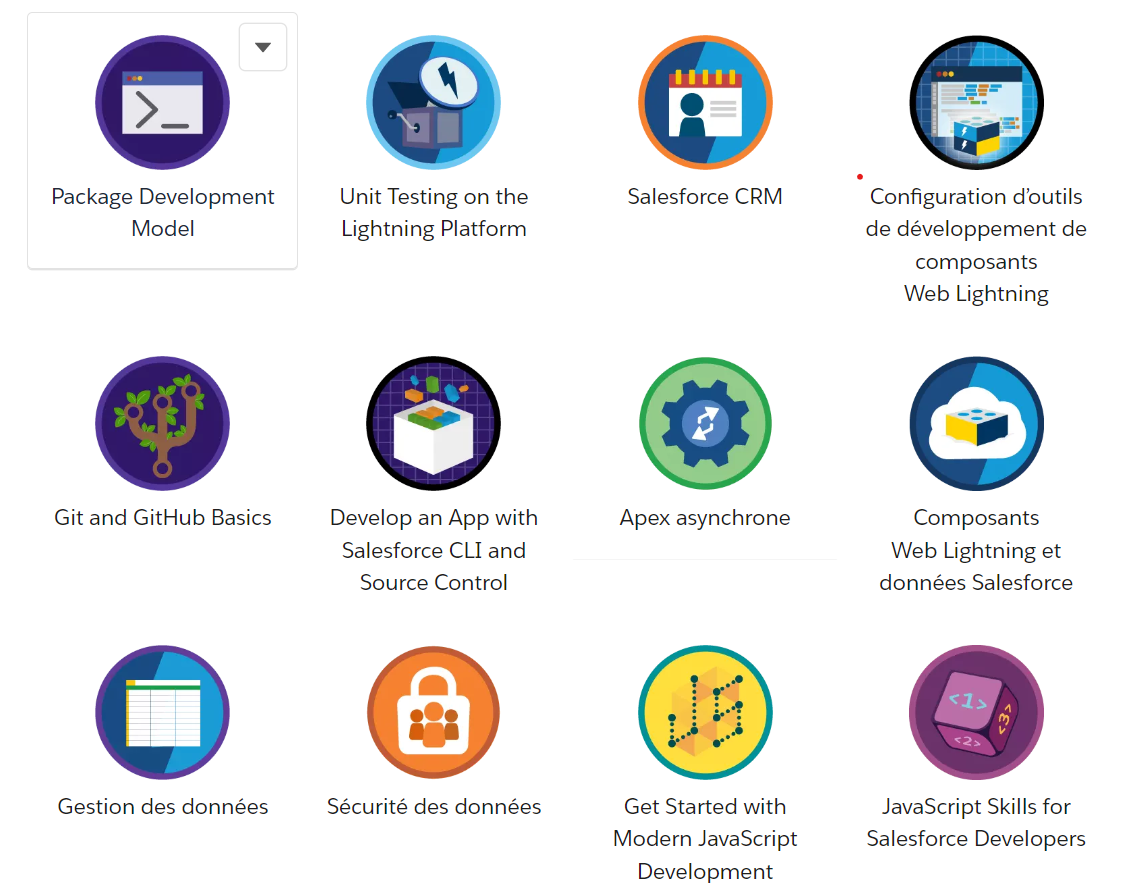
\includegraphics[width=12cm]{img/badgeSlf.png}
  \caption{Certains des badges que j'ai pu acquérir au cours de ma formation}
\end{figure}

\section{Documentation de l'entreprise avec Confluence}
Afin d'aider les employés et les futurs employés, \gz{} utilise un outil appelé Confluence, où l'entreprise peut créer des documents afin de donner une explication sur certains sujets à connaître afin de développer, ou de tout simplement connaître un sujet important. Ce sont des membres de l'entreprise qui créent les documents, afin d'aider les autres employés.

\section{Utilisation de la méthode agile avec Jira}
Jira est un système de gestion de projet. \gz{} l'utilise pour gérer et planifier les tâches à réaliser dans le cadre de leurs projets. Jira possède donc un système de ticket avec lesquels l'entreprise travaille afin d'assigner les différentes tâches aux développeurs. Un ticket est composé d'un titre et d'une description devant refléter à tout moment le problème à résoudre et la solution finalement apportée. La bonne pratique pour rédiger un ticket d'anomalie est de décrire : 
\begin{enumerate}
    \item Les étapes nécessaires pour reproduire systématiquement le défaut, avec tous les éléments de contexte pertinents.
    \item Le résultat attendu
    \item Le résultat obtenu
\end{enumerate}

Chaque ticket possède un état, en effet, un ticket peut être "à faire", peut être une "idée", peut être "en cours", peut être "terminé", ou encore en "revue de code", etc. Il y a un système logique de changement d'état. On ne peut pas passer l'état d'un ticket de "à faire" à un état "terminé", il doit d'abord passer par l'état "en cours".

~\\\indent Il est possible d'estimer le temps de réalisation d'un ticket afin d'obtenir un suivi temporel des différentes tâches d'un projet, pour pouvoir par la suite mieux estimer certaines tâches. On peut également donner une priorité à une tâche. On a les différentes priorités suivantes : 
\begin{enumerate}
    \item Lowest (priorité la plus basse)
    \item Low (priorité basse)
    \item Medium (priorité moyenne)
    \item High (priorité élevée)
    \item Highest (priorité la plus élevée)
\end{enumerate}

\section{Le projet Gespat}
\subsection{Prise en main du projet Gespat}
Lors de la deuxième semaine du stage, nous avons visionné une vidéo sur laquelle on devait se baser afin de commencer notre application ``Gespat''. C'est avec Abdelkader que j'ai été assigné au projet, ainsi qu'avec Oliver qui a pour responsabilité de nous encadrer et de prendre un rôle de chef de projet. Le premier visionnage de cette vidéo avait pour but de nous préparer avec Abdelkader vis-à-vis du cadre et des différentes problématiques du projet, avant de pouvoir écouter Antoine, le directeur, lors d'une première réunion, qui a pour but de nous présenter le projet. 
~\\\indent Suite à la réunion, on sait donc que ce projet sera un outil de relation clientèle pour gestionnaires de patrimoine. Cet outil permettra de mieux suivre les différents clients, leurs dossiers et faits de vie, et permettra une communication plus facile. Le projet se décompose en deux parties : une première partie qui vise le gestionnaire de patrimoine lui-même et une deuxième partie qui est un “espace client”, permettant au client du CGP de déposer des fichiers, de faire des demandes etc. Les premiers objectifs de livraison sont pour le salon Patrimonia, qui a traditionnellement lieu en Septembre. Cela permettra de démontrer les fonctionnalités de l’outil à un grand nombre de clients potentiels. 
~\\\indent Lors de la réunion, nous avons revisualisé la vidéo avec les membres du projet et Antoine, afin qu'il puisse s'attarder et s'arrêter sur certains points importants à reproduire. Sur la page d'un compte individuel, Antoine a premièrement souligné qu'il voudrait intégrer l'ensemble des éléments financiers, mais également les dernières et prochaines interactions que le gestionnaire de patrimoine a eu et va avoir avec son client, ainsi qu'un suivi des différents évènements de vie du client. Voici une capture d'écran de la vidéo sur laquelle se baser et qui montre quelques éléments sur lesquels Antoine veut s'inspirer ou même les reproduire.


On peut notamment y voir en haut une sorte de suivi des évènements de vie qu'Antoine veut justement reproduire sur notre projet. On peut également voir en bas à droite le suivi des interactions entre le gestionnaire et le client qu'Antoine veut également avoir sur Gespat. Il veut de plus avoir une vision de l'équipe du compte comme sur la vidéo, c'est-à-dire qu'on puisse voir les différentes personnes s'occupant du client en question. Il voudrait également voir une vision des différentes entreprises et foyers du clients.
~\\\indent Cependant, selon l'expérience d'Antoine et d'Oliver sur \slf{}, la plupart de ces éléments peuvent être reproduits et paramétrés facilement car ce sont des \textit{composants standards} de \slf{} et déjà déposable directement sur notre application à travers l'outil de modification de page de celui-ci, dont on a parlé précédemment dans la partie 1.3.1.

\clearpage

\chapter{Développement du projet Gespat et développements annexes}

\section{Les premières formes du projet}
\slf{} ayant comme philosophie de faciliter le travail des développeurs en privilégiant le \textit{low-code}, avec Abdelkader, nous avons commencé par essayer de voir les différents composants standards que l'on pouvait utiliser pour notre application. C'est alors que l'on s'est rendu compte que la plupart des composants que l'on pensait standard de part leur forme commune à \slf{}, étaient en fait inclus dans une application développé et vendu par Salesforce, qui a pour nom \textit{Financial Services Cloud}. C'est une solution de gestion de la relation client (CRM) qui aide lesentreprises du secteur financier à gérer les références, les documents, les tâches et plus encore. En résumé c'est une licence payante additionnelle de \slf{} qui rajoute des
fonctionnalités afin d'améliorer la gestion de relation client.
~\\\indent De ce fait, nous avons avec Abdelkader et Oliver, chacun a pris une version d'essai de FSC (Financial Services  Cloud) afin de voir s'il était nécessaire de l'utiliser pour notre projet, ou si on allait pouvoir tout recréer de A à Z. L'idée était d'utiliser l'organisation d'Oliver comme celle de production, et celle d'Abdelkader et la mienne comme des organisations \textit{Sandbox} sur lesquelles développer et concevoir les différentes pages de l'application. 
~\\\indent Sur FSC, beaucoup de composants, que l'on a vu dans la vidéo sur laquelle on s'est basé, sont présents. Ainsi, on peut utiliser les outils low-code de \slf{} pour les configurer et les placer sur notre application. Il y a par exemple le composant qui retrace les évènements de vie du client. Il utilise, en l'occurrence, des objets qui sont en base de données présents sur FSC mais pas présents sur \slf{}.
~\\\indent Le premier objectif était de reproduire la page d'un compte personnel comme on l'avait vu sur la vidéo, pour voir si il était possible de l'implémenter avec les composants de FSC. Nous avons donc pu donné une vision d'ensemble du client du gestionnaire de patrimoine, en montrant les informations importantes du client, ses informations financières, ses évènements de vie, etc.
~\\\indent Ensuite, nous avons pu commencer la page d'une \textit{opportunité}, et également avancer dans la traduction des éléments de FSC qui ne sont pas traduits en français. Une opportunité est un dossier, qui définit une opportunité d'investissement pour le client, on peut y retrouver son sujet, sa probabilité de réussite (selon le gestionnaire de
patrimoine), ou encore le montant de l'investissement prévu.
~\\\indent Par la suite, j'ai pu configurer et placer les différents composants de la page des pistes. Une piste est une personne, qui selon le gestionnaire de patrimoine, pourrait devenir cliente. La page d'un enregistrement d'une piste ressemble donc à celle d'un compte. Ainsi, l'objectif pour le gestionnaire est de les convertir en client, pour qu'ils aient un compte personnel à leur nom.


\section{Gestion des droits}
Ayant maintenant une base de notre application, il faut gérer les droits des utilisateurs.
En effet, depuis le début, nous avons utilisé le profil d'administrateur système pour tester les fonctionnalités de notre outil. C'est pourquoi nous devions remédier à cela et prévoir les droits des futurs utilisateurs pour éviter qu'il ne puisse faire ce qu'ils veulent.
~\\\indent Le partage de données \slf{} permet d'exposer des jeux de données spécifiques à des individus et des groupes d'utilisateurs. Les ensembles d'autorisations, les groupes d'ensembles d'autorisations et les profils fournissent une sécurité au niveau de l'objet et au niveau du champ en contrôlant l'accès. Les paramètres de partage au niveau de l'enregistrement, les rôles utilisateur et les règles de partage de l'organisation contrôlent les enregistrements individuels que les utilisateurs peuvent consulter et modifier.
~\\\indent C'est pourquoi, nous avons créer un profil d'utilisateur dans le rôle d'un gestionnaire de patrimoine, dans le but de définir et de créer des ensembles de permissions, afin de gérer leur rôle et de s'assurer que l'utilisateur ait le droit de lecture et d'écriture uniquement sur les données auxquels il est censé accéder. 

\section{Saisie des données du client}

Suite à une première démonstration de l'outil Gespat à Antoine, il a été convaincu d'utiliser FSC et de ne pas démarrer de 0 le projet et devoir faire plusieurs choses qui auraient été encombrantes et longues à faire par rapport à la plus-value apportée. De plus, il nous a conseillé d'utiliser \textit{FormAssembly}, afin de créer un formulaire connecté à notre outil Salesforce, dans le but que le client y remplisse ses informations nécessaires à l'analyse du gestionnaire de patrimoine. Cela lui permettrait de gagner du temps, et de ne pas avoir besoin de remplir les données de ses clients un par un. Le but secondaire du formulaire, serait de pouvoir connaître la connaissance et l'expérience en investissement du client, pour pouvoir faire traduire cela à travers un score financier.

\subsection{FormAssembly}
FormAssembly est la solution de formulaire nº1 pour \slf{} conçue pour aider les équipes à rationaliser les processus complexes et à générer des conversions de formulaires de qualité.
Grâce à mon collègue Tristan déjà à l'aise avec FormAssembly et grâce à quelques tutoriels, j'ai pu me former à son utilisation et à son intégration avec \slf{}. Antoine nous ayant indiqué qu'il voudrait un formulaire de recueil d'informations du client. Pour ce faire, j'ai pu implémenter un formulaire, qui demande au client :
\begin{enumerate}
    \item Ses informations personnelles
    \item Ses informations familiales et matrimoniales
    \item Ses informations professionnelles
    \item Les projets qu'il souhaite réaliser (constitution d'une épargne, préparation de sa succession, etc)
    \item Son niveau en finance et des questions sur la finance
    \item Son avis sur le niveau de risque que représentent certains investissements
\end{enumerate}

Pour que le client accède au formulaire, il est prévu que le gestionnaire de patrimoine prenne d'abord contact avec un client. Il suffit que le client lui donne son nom, son prénom et son adresse e-mail. Ensuite, sur la page d'accueil de notre application, Abdelkader a créé un \textit{composant web LWC} sur lequel j'ai pu également travaillé. Ce composant permet au gestionnaire de patrimoine d'entrer le nom, le prénom et l'adresse e-mail d'un client, afin de créer un compte personnel dans la base de données. Après la soumission de ces informations dans le composant, un e-mail est automatiquement envoyé à l'adresse e-mail du client, avec un lien du formulaire. Les informations déjà entrées en base de données (nom, prénom, e-mail) sont pré remplies par le formulaire.

\begin{figure}[!ht]
  \centering
  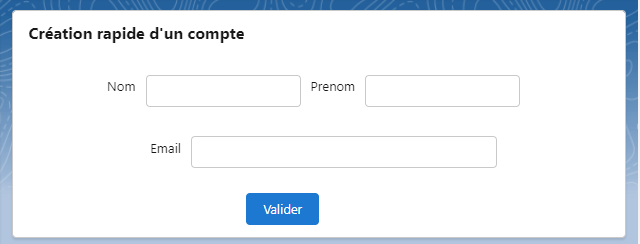
\includegraphics[width=15cm]{img/QuickAccountCompo.png}
  \caption{Capture d'écran du LWC qui permet de créer un compte rapidement}
\end{figure}


\section{Conception du formulaire de recueil d'informations client pour Gespat}
 \subsection{Problème}
 Le recueil et le suivi des informations des clients des gestionnaires de patrimoine peuvent être redondants. C'est pourquoi, Antoine a vu le besoin de concevoir un formulaire qui recueille les informations du client pour le gestionnaire de patrimoine.
 \subsection{Solution}
 C'est ainsi qu'après quelques recherches et après une suggestion du directeur Antoine, j'ai décidé de concevoir ce formulaire sur FormAssembly. Ce formulaire est extérieur à \slf{} mais connecté à celui-ci.
 
 \subsubsection{Conception du formulaire}
 Premièrement, il faut élaborer la partie visuelle du formulaire. Pour cela, FormAssembly propose d'ajouter le type de champ de saisie que l'on veut. Il est possible d'ajouter à son formulaire un champ de saisie de texte, une zone de texte, des cases à cocher, des listes de sélections, etc. Il faut nommer ces champs, non seulement pour que l'utilisateur comprenne ce qu'il doit renseigner dans le champ, mais également afin que l'on puisse connecter ces champs à notre application sur \slf par la suite. On a la possibilité de placer ces champs comme on le souhaite, que ce soit dans des sections particulières ou non. On peut rendre répétable ou obligatoire n'importe quel champ ou n'importe quelle section. 
 ~\\\indent De ce fait, j'ai pu dans un premier temps créer et placer les champs en rapport avec les informations personnelles du client sur une première page. Sur une deuxième page, le client doit renseigner ses informations professionnelles et doit par exemple indiquer son emploi, son type de contrat de travail, ou encore ses revenus annuels et mensuels. Sur la prochaine page, le client renseigne les différents projets qu'il veut réaliser. Sur la quatrième et la cinquième page, le client doit répondre à un questionnaire sur ses connaissances financières mais également sur ses connaissances par rapport aux différents risques sur certains investissements.
 
 \subsubsection{Lien avec \slf{} et connecteurs}
 Suite à la conception visuelle du formulaire, il est nécessaire que les réponses des clients à celui-ci se traduisent sur notre application \slf{}. Or, FormAssembly se marie parfaitement et est conçu notamment pour \slf{}. L'outil propose donc un système de connecteurs qui va lier les champs du formulaire à ceux de \slf{}. FormAssembly offre trois différents types de connecteurs, un qui pré-remplit le formulaire, un autre qui envoie des informations du formulaire à \slf{} à la soumission du formulaire par l'utilisateur, et un autre qui envoie des informations du formulaire après la soumission de celui-ci.
 ~\\\indent Grâce au connecteur de pré-remplissage, je peux récupérer le nom, le prénom et l'adresse mail du client et les pré-remplir sur le formulaire. Cela peut se faire grâce au composant présent sur la page d'accueil qui permet de créer un compte rapidement. En effet, une fois les champs du composant remplis et acceptés, il va envoyer un e-mail contenant le lien du formulaire au client. Or, dans ce lien est présent l'ID unique du compte fraîchement créé avec le composant. Je le référence donc sur le connecteur de pré-remplissage et peut donc aller chercher les informations spécifiques à cet ID unique.
 ~\\\indent FormAssembly est connecté à la base de données de l'organisation \slf{} que l'on souhaite. Ainsi, avec le connecteur d'envoi d'informations lors de la soumission du formulaire, je peux connecter chaque champ du formulaire en les liant au champ de \slf{} de mon choix. Dans mon formulaire, je choisis de mettre à jour un objet de type Compte personnel, si toutefois un enregistrement avec l'ID que l'on a été chercher dans le lien est trouvé. Si ce n'est pas le cas, un nouvel enregistrement de Compte personnel est créé. Antoine ayant demandé de recueillir certaines informations spécifiques au besoin d'un gestionnaire de patrimoine, j'ai dû créer des nouveaux champs principalement sur l'objet "Compte". J'ai pu également ajouter des types d'évènements possibles sur l'objet "Évènement de vie". Sans la création des différents champs nécessaires, il n'était pas possible de lier certains champs du formulaire à des objets sur \slf{}. Lors de la soumission du formulaire par le client, je crée plusieurs objets. Comme indiqué précedemment, un compte est mis à jour s'il existe et créé s'il n'existe pas, un compte est créé si le client est marié/pacsé, puis un compte est créé pour chaque enfant. De ce fait, des relation entre ces comptes sont créées afin que le gestionnaire puisse avoir une vision du foyer du client si toutefois il possède des enfants à charge et un compagnon.



\section{Affichage des données du client}
Avec toutes ces informations que le client a fourni, il faut maintenant les afficher sur notre application.

\subsection{Les composants standards}
Pour concevoir une page web, \slf{} utilise une technologie particulière. En effet, au lieu de développer et de concevoir une page entière, sur \slf{}, une page est composée de plusieurs éléments mis bout à bout que l'on appelle composants Lightning. On peut en développer de façon personnalisée (LWC), ou bien reprendre et réutiliser les composants déjà conçus par \slf{}. Ce sont les composants standards ou composants Lightning standards. 
~\\\indent Grâce à cela, certaines données sont déjà prises en compte et facilement affichable avec ces composants standards. Ainsi, par exemple sur Gespat, les informations personnelles des clients du gestionnaire de patrimoine, les opportunités (dossiers) de celui-ci, ou encore ses rapports et ses tableaux de bord sont présentables sur l'application grâce aux composants standards.
~\\\indent  C'est donc avec l'éditeur de page d'application de \slf{}, que pour construire une page web, il faut assembler plusieurs composants qui chacun font une action particulière.
\newpage

\subsection{Les composants web LWC}
 Pour les champs déjà présents de façon standard sur \slf{}, les composants standards les présentent déjà bien. Cependant, il est nécessaire pour certaines informations, et certains champs personnalisés par exemple, de créer ses propres composants personnalisés. On les appelle les \textit{LWC} (Lightning Web Components).
 ~\\\indent Pour \slf{}, au lieu de coder ou concevoir une page entière, il est plus simple de développer des composants LWC, qui sont des éléments d'une page que l'on peut déposer côte à côte entre eux, pour au final former une page web. Un LWC utilise de l'\textit{HTML} et du \textit{CSS} pour l'esthétique et l'apparence de la page, et utilise du \textit{Javascript} pour effectuer des calculs ou communiquer avec du code Apex qui lui va chercher des informations en base de données.
 ~\\\indent C'est donc grâce à cette technologie, qu'avec Abdelkader nous avons pu afficher les informations de connaissance financière du client que l'on a pu récupérer grâce au formulaire de recueil d'informations de FormAssembly. Il a fallu d'abord créer un objet de connaissance financière qui répertorie les réponses aux questions du formulaire lié à la finance et au risque d'investissement. Ainsi, d'un autre côté, un score de connaissance financière et un score de connaissance du risque d'investissement est établi et calculé grâce aux réponses aux différentes questions du formulaire. Ensuite, en fonction des différents scores du clients, on indique au gestionnaire de patrimoine si le client est novice, si il a un niveau intermédiaire ou expert.

\begin{figure}[!ht]
  \centering
  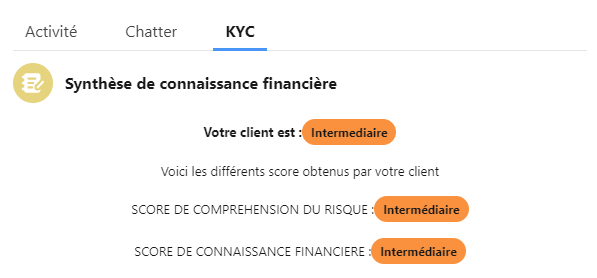
\includegraphics[width=15cm]{img/SyntheseFinanciere.png}
  \caption{Capture d'écran du LWC de synthèse de connaissance financière du client}
\end{figure}


\section{Déploiements}
Comme je l'ai précisé précédemment dans la partie 2.2, pour concevoir et développer l'outil Gespat, nous avons avec Oliver et Abdelkader chacun une organisation. Or, l'organisation d'Oliver étant celle de production, et celle d'Abdelkader et la mienne celles de développement, il faut déployer les travaux réalisés sur les organisations de développement sur celle de production, lorsque l'on s'est assuré que ces travaux fonctionnaient d'abord sur les organisations de développement.
\subsection{Plugin \slf{} sur Visual Studio Code}
\slf{} a développé un plugin sur Visual Studio Code. Ce plugin qui est le SFDX CLI (Salesforce Developer Experience Command Line Interface), est un outil en ligne de commande permettant de faire des développements Salesforce.
 ~\\\indent Grâce à ce plugin, pour le développement de Gespat, on se connectait aux organisations de développements, récupérant le travail fait sur celles-ci en récupérant leurs données et \textit{meta-données}. Ensuite, il faut créer une version de paquet contenant les différentes données et meta-données de l'organisation de développement, afin d'ensuite l'installer sur l'organisation de production. Tout cela était réalisé en utilisant des "commandes SFDX" (des commandes issues du plugin \slf{})
 
 \section{Résultats}
 Pour l'instant, notre outil n'est pas encore utilisé par des vrais utilisateurs. Le but est d'intégrer notre application Gespat au projet principal de l'entreprise qu'est Shaker Data. Or, notre outil utilisant une licence additionnelle de \slf qui est Financial Services Cloud, des problèmes d'intégration s'opposent à nous. En effet, plusieurs éléments de notre projet ne sont pas reconnus sur l'organisation de Shaker Data. Ce qui implique que l'intégration de l'outil Gespat est encore en cours et donc pas utilisable pour l'instant.
 ~\\\indent Cependant, lorsque l'intégration sera terminée, le gestionnaire de patrimoine pourra avoir une vision globale de ses clients, en ayant à disposition ses informations principales, son niveau de connaissance financière, son niveau de connaissance des différents risques d'investissements sans même qu'il n'ait à analyser quoi que ce soit. D'un autre côté, il pourra entrer manuellement les informations financières de son client, car la page d'un compte personnel d'un client dispose de composants standards qui montre les différents soldes des comptes financiers du client.
 
\section{Développements annexes sur Shaker Data}
 \subsection{Méthodologie et étapes de développement sur Shaker Data}
 \gz{} possède une méthodologie de travail à suivre lorsque l'on développe. Une tâche est à réaliser, on crée donc un ticket sur Jira qui explique la tâche à réaliser. L'entreprise travaille bien évidemment avec \textit{Git} afin d'avoir un suivi et un système de gestion de versions de leurs différents projets. 
 ~\\\indent De ce fait, après qu'un développeur ait été assigné à un ticket, il doit tirer une \textit{branche} sur la branche de développement courante sur Git, sur laquelle il va pouvoir développer isolément, afin de ne pas entrer en conflit avec les autres développements. Cette branche est donc dédié au développement en cours. Ensuite, le développeur doit créer une organisation Scratch pour le travail du ticket. Cela permet notamment d'éviter des problèmes de synchronisation. Il va donc développer autant que possible sur cette scratch, de manière à pouvoir apporter des modifications mineures facilement et rapidement. Une fois les développements terminés et les tests unitaires du projet validés, le développeur doit générer une version de paquet et l'installer sur une organisation sandbox du projet. Cette installation permet de tester les développements réalisés en conditions réelles. En outre, cette installation sur sandbox permet de détecter les différents problèmes possibles liés au déploiement. Ensuite, une fois que l'on est sûr que tous les développements sont fonctionnels et stables, il est nécessaire de lancer l'ensemble des tests unitaires du projet, afin de de vérifier que notre travail n'a pas "cassé" celui-ci. Dans la mesure où ces tests unitaires passent, il faut ouvrir une \textit{Pull Request} sur Git afin de fusionner le code développé avec la branche de production. Une fois la Pull Request acceptée par celui en charge du projet, on peut fermer le ticket.
 
 \begin{figure}[!ht]
  \centering
  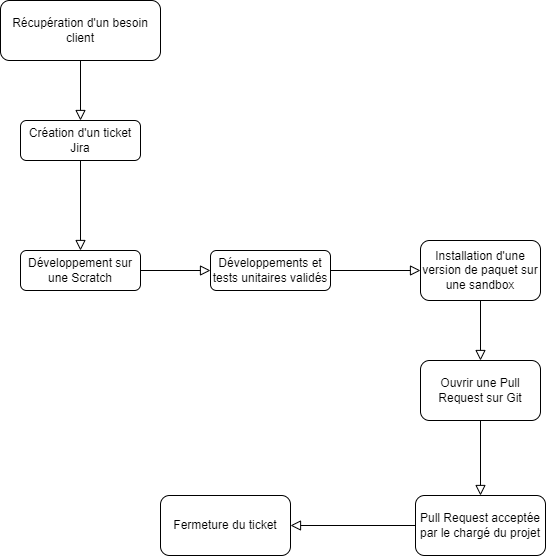
\includegraphics[width=15cm]{img/schemaEtapesDev.drawio.png}
  \caption{Schéma des étapes de développements de l'entreprise}
\end{figure}
\clearpage
 
 
 \subsection{Refactorisation et tests unitaires d'une classe Apex}
 Une fois que j'ai pu comprendre et assimiler cette méthodologie, Samuel m'a confié un ticket. Le but était de créer des tests unitaires sur une classe Apex sur le projet principal de \gz{}, mais également de la \textit{refactoriser}. Il y a plusieurs objectifs lors de la création de tests unitaires. Cela permet de trouver des bugs ou améliorer la structure du code. Mais un point très important pour \gz{} est le filet de sécurité. C'est-à-dire que lorsque l'entreprise fera des changements ultérieurement, elle verra tout de suite si ces changements apportent des régressions.
 Avant de pouvoir commencer à travailler sur le ticket, j'ai du suivre un module de formation sur Trailhead afin de comprendre comment bien effectuer des tests unitaires sur les classes Apex. Après cela, j'ai pu commencer à réellement commencer le développement des tests unitaires et sur la refactorisation de la classe "RuleTAEG". 
 ~\\\indent Cette classe est une des nombreuses "Rule" du projet EDF, elle permet donc que l'on s'appuie sur celle-ci afin de faire fonctionner l'outil Shaker Data. Les "Rule" sont donc des règles que l'outil doit suivre afin d'être cohérent dans tous ses calculs financiers vis-à-vis non seulement de la loi, mais également afin d'arriver à un calcul final correct. La classe RuleTAEG, en l'occurrence, permet de calculer le TAEG (taux annuel effectif global), il représente le coût total du crédit pour le consommateur. Il est exprimé en pourcentage annuel du montant total du crédit. Il s’agit du montant que vous devrez verser en plus de la somme empruntée. Il est alors important de réaliser des tests unitaires sur les "Rule" de Shaker Data, afin de s'assurer que celui-ci fonctionne correctement. De plus, afin de déployer en production, \slf{} requiert qu'il y ait une couverture de tests sur le code d'au moins 75\%. Si ce n'est pas le cas, impossible de déployer. 
 \subsubsection{Documentation de la classe}
La classe n'étant pas documentée, j'ai pu demander de l'aide à l'auteur de la classe, Samuel, qui a pu m'aiguiller sur les différentes utilités des différentes méthodes de celle-ci. Cela m'a permis de documenter la classe afin que les futurs développements sur celle-ci soient facilités. Pour cela, j'ai pu documenter chaque méthode de la classe en expliquant pour chacune des méthodes, ce que faisait celle-ci, ce qu'elle retournait et quelle était l'utilité et la signification de chacun de ses paramètres. Pour cela, Apex utilisant une syntaxe semblable à Java, j'ai pu utilisé les standards Java, avec notamment quelques Tags de documentation. Pour la valeur de retour, j'ai utilisé le tag "@return", pour les paramètres de la méthode j'ai pu utilisé le tag "@param", et enfin grâce au tag "@see", j'ai fait référence aux autres méthodes utilisées. Grâce à cette documentation, lors du survol de la souris sur une méthode, une info-bulle affiche la documentation de celle-ci. Cela permet aux futures personnes qui vont s'occuper de la classe, de comprendre facilement comment utiliser chaque méthode.
\subsubsection{Tests Unitaires}
Afin de réaliser les tests unitaires de la classe, j'ai du refactoriser la classe en extractant des bouts de méthodes dans des autres méthodes. En effet, certaines fonctions étaient assez longues et prenaient plus de 50 lignes de code. Or, il est plus difficile et lourd de tester unitairement une longue méthode floue faisant plusieurs choses à la fois, plutôt qu'une courte méthode claire et concise qui fait une seule chose précise et bien. De ce fait, la refactorisation du code de la classe m'a aidé à tester celle-ci, en me permettant de me concentrer sur le test de plusieurs courtes méthodes faciles à tester une par une, au lieu de devoir tester une longue méthode encombrante.
~\\\indent Lorsque l'on crée une méthode de test, on crée d'abord des données à tester. Ensuite on va appeler la méthode à tester et stocker le résultat de cette méthode dans une variable. Pour enfin, vérifier que le résultat de la méthode est bien égale à la valeur attendue.
Pourtant, certaines méthodes possèdent plusieurs alternatives (plusieurs if ou else if). Afin de tester efficacement ces différentes alternatives, j'ai créé pour chacune une méthode de test. Cela permet de tester efficacement et de cibler les bouts de code à tester.
~\\\indent Après exécution des tests, on peut visualiser quelles portions de code sont couvertes par les tests, et lesquelles ne le sont pas. Cela permet d'identifier du code mort (une portion du code qui ne s'exécutera jamais), ou des cas qui ne sont pas testés. Lors de l'exécution de ma classe de test sur la RuleTAEG, j'ai constaté une couverture de code de 96\%.



\SpecialSection{Conclusion}
Avec l'aide des différents outils de gestion de relation et client et la plate-forme de développement de \slf{}, j'ai pu concevoir et développer, en équipe, un outil facilitant le travail des gestionnaires de patrimoine en proposant un suivi personnel et financier de leurs clients.
~\\\indent Lors de ce stage j'ai donc pu acquérir de nouvelles connaissances ainsi que de nouvelles compétences. En effet, j'ai découvert \slf{} et l'outil de gestion de relation client qu'il est, ainsi que sa plateforme de développement. En outre, j'ai pu mettre en pratique la méthode agile ainsi que les bonnes pratiques de code. En effet, ayant travaillé au long du stage au sein d'une équipe de développeurs, j'ai été forcément amené à retravailler du code qui n'était pas le mien. C'est grâce à cela que j'ai compris combien il était important de structurer et de documenter son code, comme j'ai pu l'apprendre lors du DUT, afin que les prochaines personnes qui le retravaille puisse le comprendre facilement. Cela permet un gain de temps non négligeable sur les développements de chacun. Grâce à l'apprentissage de l'outil Git lors de mes études, j'ai pu facilement assimiler son utilisation au sein de l'entreprise. Mais aussi, l'enseignement de la méthode agile m'a permis de rapidement comprendre la méthodologie de travail de \gz{} à travers sa planification et sa quantification du temps de travail des tâches de chacun. Pour finir sur ce parallèle entre mon stage et ma formation à l'IUT, j'ai pu réutiliser mon apprentissage de différents langages lors du DUT. J'ai pu utilisé du JavaScript, de l'HTML et du CSS mais il y a également l'enseignement du Java que j'ai pu retranscrire en programmant en Apex.
~\\\indent Cette expérience m'a conforté dans l'idée de vouloir continuer l'an prochain vers une licence professionnelle dans le développement Web en alternance, afin de pouvoir continuer mes études tout en acquérant de l'expérience professionnelle. 

\bibliographystyle{myunsrt}
\small
\bibliography{rapport}
Site d'une agence d'intérim/cabinet de recrutement https://www.manpower.fr/ \newline
https://www.journaldunet.fr/ \newline
wikipedia.org \newline
https://developer.mozilla.org/


\Annex{Annexe 1}
\begin{figure}[!ht]
  \centering
  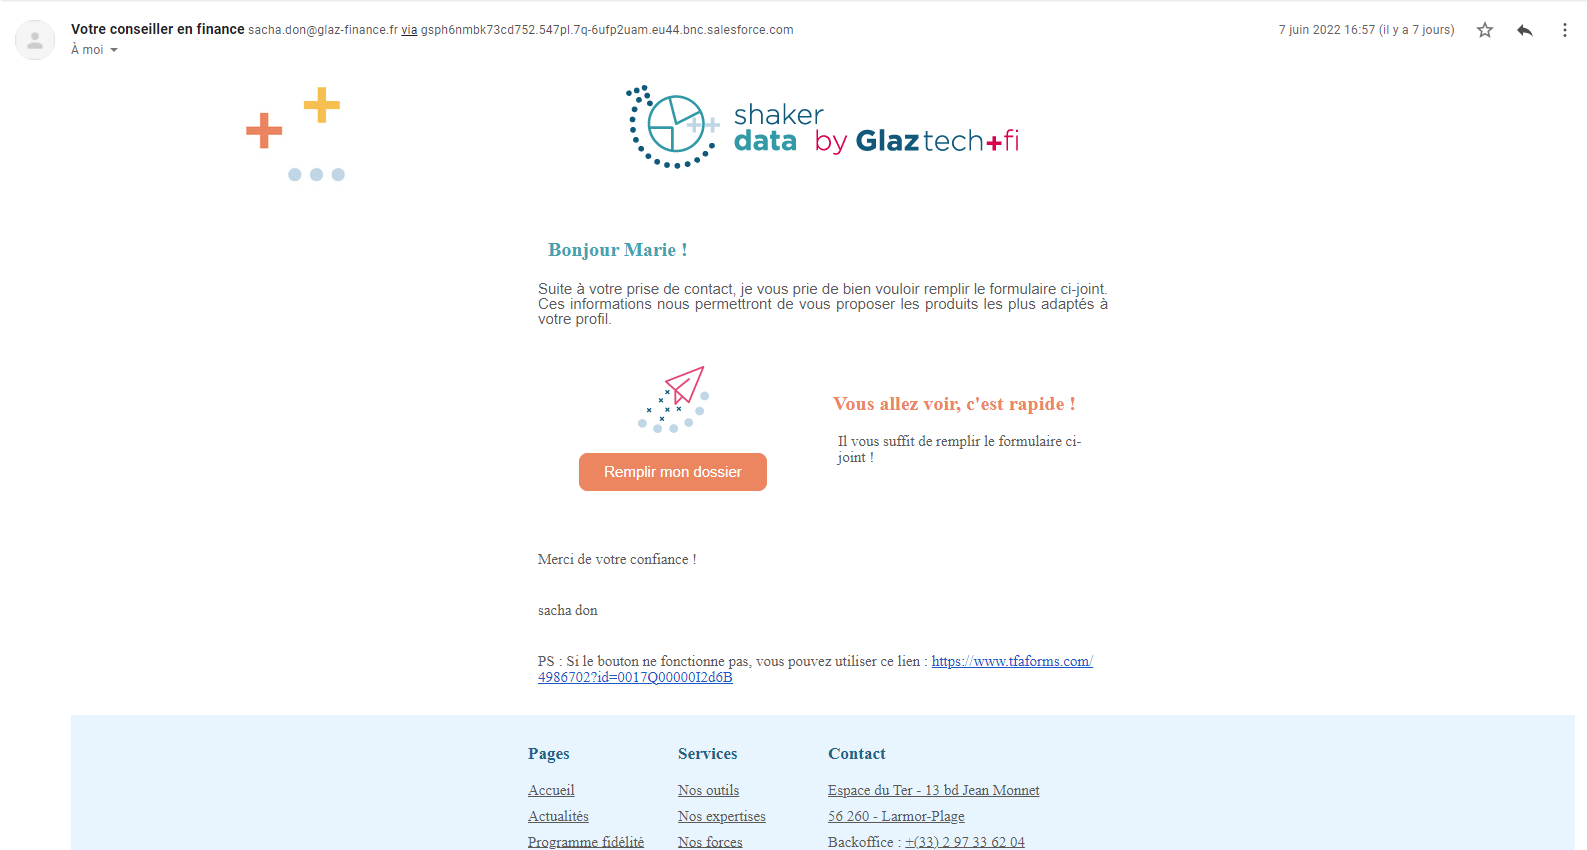
\includegraphics[width=15cm]{img/emailQuickAccount.png}
  \caption{Capture d'écran de l'e-mail envoyé lorsque le gestionnaire remplit le composant ci-dessus}
\end{figure}
\newpage
\Annex{Glossaire}
    \textbf{Gestionnaire de patrimoine} : Le conseiller de gestion en patrimoine gère les actifs de ses clients. C’est un spécialiste de l’investissement qui a pour rôle de fournir des programmes sur mesure à ses clients pour préserver ou accroître leur patrimoine.\newline
    
   ~\\\indent \textbf{Courtier immobilier} : Un courtier en financement immobilier est un intermédiaire entre une banque et un particulier en quête d’un crédit immobilier pour financer l’acquisition de son bien.\newline


    ~\\\indent \textbf{FinTech} est un terme créé par la fusion des mots "finance" et "technologie". Il désigne une entreprise de type start-up, proposant des services financiers en s'appuyant sur les nouvelles technologies numériques. \newline


    ~\\\indent Un \textbf{apporteur d'affaires} est une personne qui met en relation des personnes qui souhaitent réaliser entre elles des opérations commerciales. Pour l'entreprise en l'occurrence, c'est lui qui va apporter les différents dossiers de ses clients, afin que nous les traitons.\newline


    ~\\\indent \textbf{Composant standard} est un élément développé par \slf{} que l'on peut réutiliser afin de concevoir des pages web sur celui-ci.\newline


     ~\\\indent Les outils \textbf{Low Code/No Code} permettent de créer des applications (mobile ou web) ou d’automatiser des processus sans nécessairement maîtriser toutes les étapes de programmation bien souvent complexes. Ces outils sont basés sur les trois principes suivants: 
    \begin{enumerate}
        \item conception d’applications directement via des modèles
        \item La possibilité de glisser-déposer des composants applicatifs pour former des pages web
        \item génération automatique de lignes de code
        \item programmation visuelle
    \end{enumerate}
    
    ~\\\indent \textbf{Financial Services Cloud} (FSC) est une solution de gestion de la relation client (CRM) qui aide les
entreprises du secteur financier à gérer les références, les documents, les tâches et plus
encore. En résumé c'est une licence payante additionnelle de \slf{} qui rajoute des
fonctionnalités afin d'améliorer la gestion de relation client.\newline


    ~\\\indent Les \textbf{organisations Sandbox} sont des environnements \slf{} se rapprochant le plus de l'environnement de production, en effet, la Sandbox copie l'organisation de production en omettant les données présentes sur celle-ci. Cela permet donc de tester les développements en conditions réelles avant de réellement les déployer en production. Une organisation Sandbox peut être effacée lorsqu'on le souhaite.\newline
    
    ~\\\indent Les \textbf{organisation scratch}sont des organisations vides contenant aucune donnée et qui sont automatiquement effacées dans un délai de 30 jours maximum. Ce sont des environnements jetables dédié au développement, chaque développeur travaille seul sur sa scratch.\newline


    ~\\\indent Une \textbf{opportunité} est un objet sur \slf{} qui représente un dossier, qui définit une opportunité d'investissement pour le client, on peut y retrouver son sujet, sa probabilité de réussite (selon le gestionnaire de patrimoine), ou encore le montant de l'investissement prévu.\newline


   ~\\\indent \textbf{FormAssembly} est la solution de formulaire nº1 pour \slf{} conçue pour aider les équipes à rationaliser les processus complexes et à générer des conversions de formulaires de qualité.\newline


   ~\\\indent Les \textbf{LWC} (Lightning Web Components) sont des éléments HTML personnalisés qui utilise de l'HTML, du CSS et du JavaScript.\newline

  ~\\\indent  Les \textbf{meta-données} sur \slf{} sont des fichiers \textit{XML} qui représente les différents éléments qui le compose, tels que les objets, les présentations de page, les LWC, etc. Les meta-données sont donc des données qui décrivent des données.\newline


    ~\\\indent \textbf{Git} est un système de contrôle de version. Il s’agit d’un outil de développement qui aide une équipe de développeurs à gérer les changements apportés au code source au fil du temps, et à garder une trace de ceux-ci.\newline


 ~\\\indent \textbf{Branche (Git)} : Presque tous les système de contrôle de version tels que Git proposent une certaine forme de gestion de \textbf{branches}. Créer une branche signifie diverger de la ligne principale de développement et continuer à travailler sans impacter cette ligne.\newline


 ~\\\indent Les \textbf{pull requests} sur git sont une fonctionnalité facilitant la collaboration des développeurs. Elles fournissent une interface Web qui permet discuter des changements proposés avant de les intégrer au projet officiel. Une fois qu'il effectué une revue de code de la pull request, le chargé de projet s'occupe de l'accepter, ou décide demander des modifications sur celle-ci.
\newline

 ~\\\indent Le \textbf{refactoring de code} consiste à améliorer le code source d’une application informatique en le modifiant sans ajouter de nouvelles fonctionnalités et sans fixer de bugs. Cette amélioration peut consister à de la simplification pour faciliter sa maintenance ou le rendre plus générique. Le tout sans modifier le comportement fonctionnel de la solution informatique.\newline

 ~\\\indent \textbf{XML} est un langage de balisage créé pour définir une syntaxe de codage de documents que les humains et les machines peuvent lire. Pour ce faire, il utilise des balises qui définissent la structure du document, ainsi que la manière dont le document doit être stocké et transporté.\newline


     ~\\\indent Les feuilles de style en cascade, généralement appelées \textbf{CSS} de l'anglais Cascading Style Sheets, forment un langage informatique qui décrit la présentation des documents HTML et XML. Il permet ainsi de décorer ces dernières.\newline


     ~\\\indent \textbf{HTML}
    description=Le HyperText Markup Language, généralement abrégé HTML ou, dans sa dernière version, HTML5, est un langage informatique conçu pour représenter les pages web.\newline



     ~\\\indent \textbf{Javascript} est un langage de programmation qui permet d'implémenter des mécanismes complexes sur une page web. À chaque fois qu'une page web fait plus que simplement afficher du contenu statique — afficher du contenu mis à jour à des temps déterminés, des cartes interactives, des animations 2D/3D, des menus vidéo défilants, ou autre, JavaScript a de bonnes chances d'être impliqué.


\end{document}

